\documentclass[]{article}
\usepackage{graphicx}
\usepackage{amsmath}

%opening

\begin{document}

\section{Dependency Parsing}
\subsection{Dependency Grammars}
\\

Dependency grammars are a way to represent syntactic structure using a 'dependency' notion of the words themselves, without any explicit phrase structure rules.

\begin{figure}[h!]
	\begin{center}
		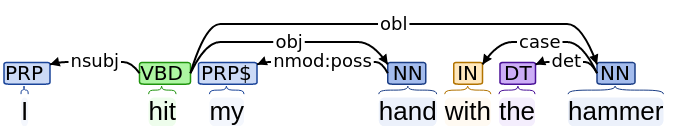
\includegraphics[width=0.6\linewidth]{./images/dependency.png}
		\label{fig:dep1}
		\end{center}
\end{figure}

\begin{center}
Figure \ref{fig:dep1}: A typical dependency parse in (CoreNLP parse)
\end{center}



\end{document}
